\documentclass[]{article}
\usepackage[brazil]{babel}
\usepackage[]{graphicx}
\usepackage{amsmath}

\title{Sistema de Alarme de Automóvel}
\author{Erickson Müller, mat: 20230001178\\ Nicole Moritz, mat: 2221101074}
\date{24 de abril de 2024}

\begin{document}
	\maketitle
	\pagebreak
	\section{Circuito}
		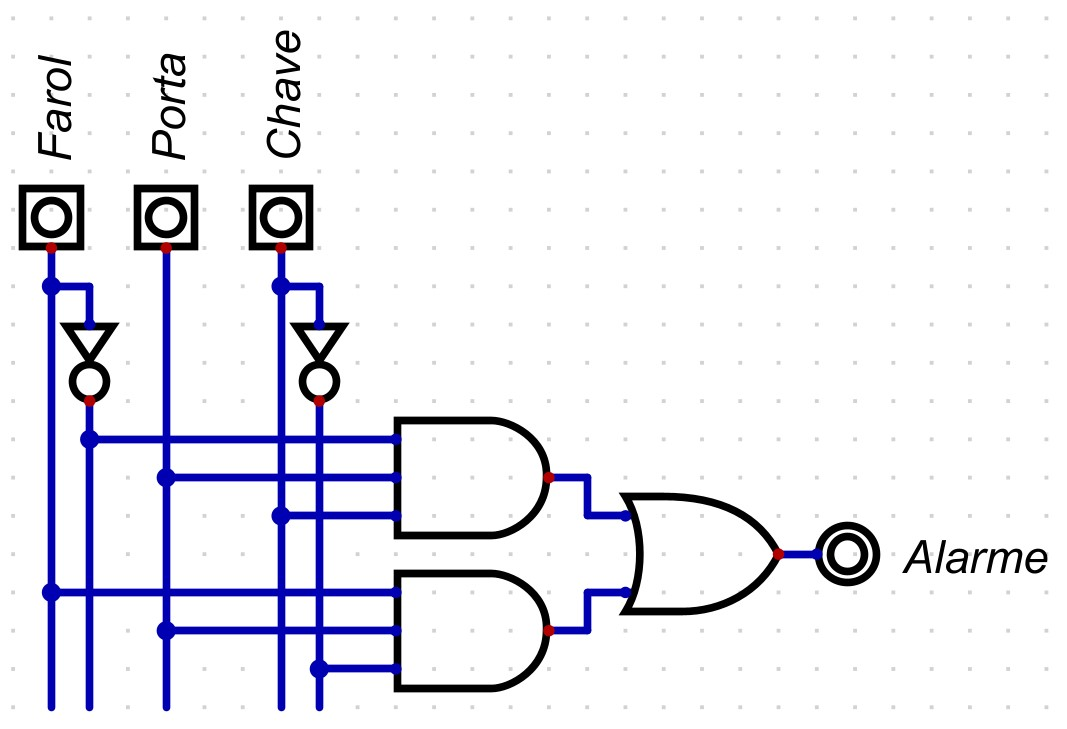
\includegraphics[scale=0.5]{Images/Circuito Alarme.jpg}
	\section{Tabela Verdade}
		\hspace*{4cm}
		\begin{tabular}{|c|c|c|c|}
			\hline
			\textbf{ F } & \textbf{ P } & \textbf{ C } & \textbf{ A } \\
			\hline
			0 & 0 & 0 & 0 \\
			\hline
			0 & 0 & 1 & 0 \\
			\hline
			0 & 1 & 0 & 0 \\
			\hline
			0 & 1 & 1 & 1 \\
			\hline
			1 & 0 & 0 & 0 \\
			\hline
			1 & 0 & 1 & 0 \\
			\hline
			1 & 1 & 0 & 1 \\
			\hline
			1 & 1 & 1 & 0 \\
			\hline
		\end{tabular}
	\\
	F = Farol \\ P = Porta \\ C = Chave \\ A = Alarme
	\pagebreak
	\section{Expressão}
		\begin{equation*}
			A = (\overline{F}.P.C) + (F.P.\overline{C})
		\end{equation*}
	\section{Circuitos Integrados}
		Além de fonte de energia, cabos diversos, switch, resistor e lâmpada LED; Foram usados neste projeto 3 peças de portas lógicas para representar o circuito:\\ \\
		CI 7400 (NAND): Foi usada para negar os sinais do farol e da chave, poderia também ser usado uma porta NOR. \\ \\
		CI 7408 (AND): Foi usada para representar as portas AND do circuito, como o circuito utiliza portas AND de 3 entradas, tivemos que utilizar 4 portas AND de 2 entradas para obter os mesmos resultados. \\ \\
		CI 7432 (OR): Foi usada ao final do circuito para representar a porta OR. \\
	\section{Processo de Montagem em Plataforma Virtual}
		\subsection{Energização da Protoboard e Montagem das Entradas}
			1 = Farol \\ 2 = Porta \\ 3 = Chaves \\
			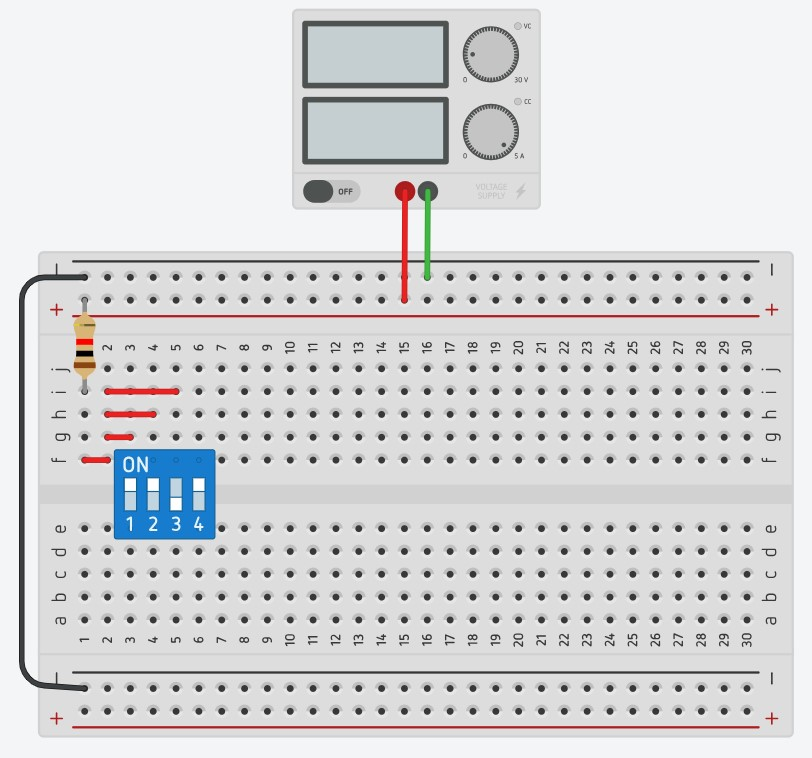
\includegraphics[scale=0.5]{Images/Tinkercad 01.jpg} \\
		\subsection{Porta Lógica NAND (CI 7400)}
			Essas portas lógicas são necessárias para inverter os valores das entradas 1 (Farol, representado pelo fio amarelo) e 3 (Chave na ignição, representado pelo fio verde) \\
			A CI foi energizada puxando da linha 2 da parte superior e aterrando no negativo da parte inferior. \\
			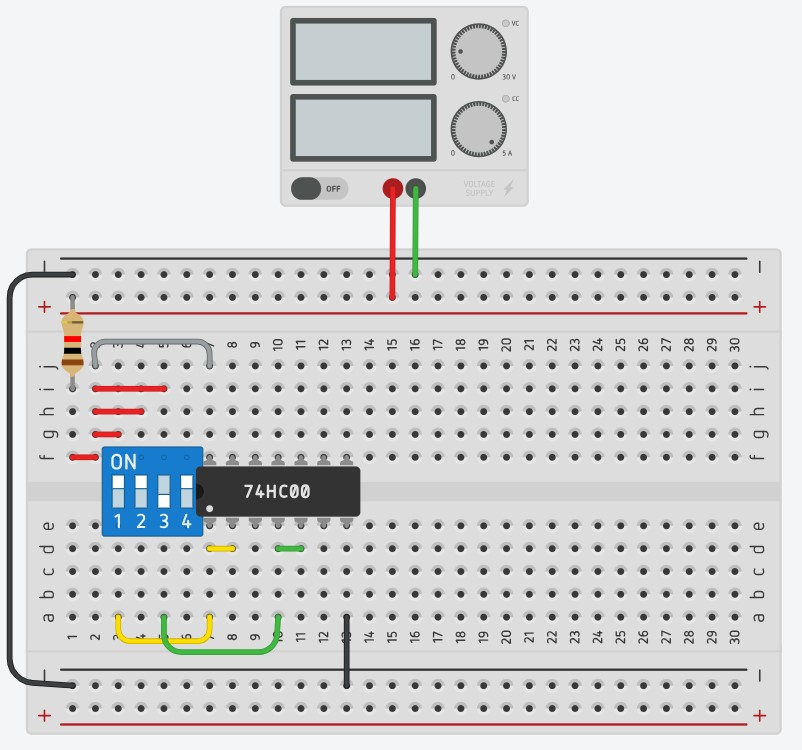
\includegraphics[scale=0.5]{Images/Tinkercad 02.jpg} \\
		\subsection{Porta Lógica AND (CI 7408)}
			Na parte inferior, foram montados duas portas AND, uma com o sinal da Porta e o sinal negado do Farol, outra com o sinal da Porta e o sinal negado da Chave. \\
			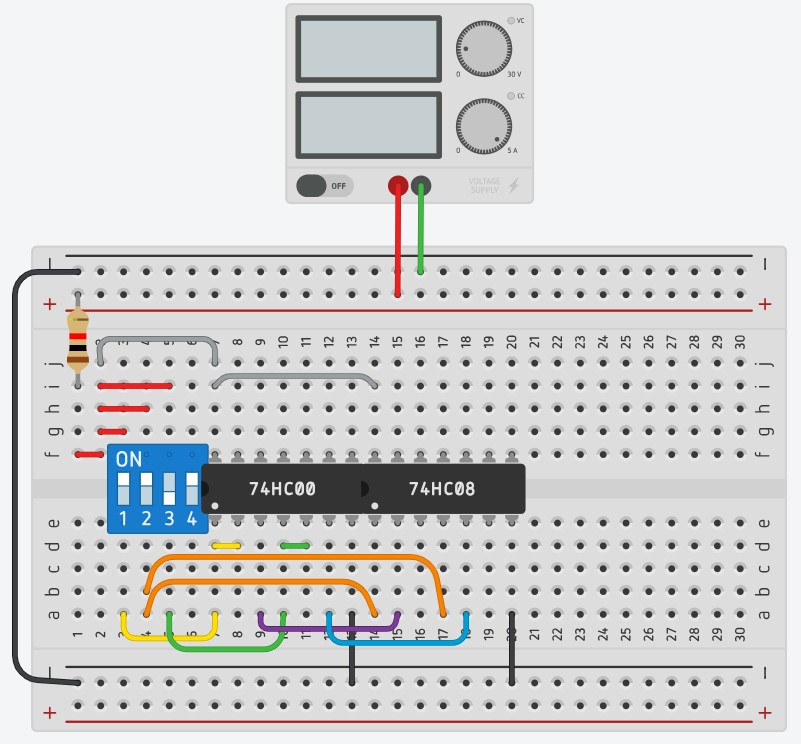
\includegraphics[scale=0.5]{Images/Tinkercad 03.jpg} \\
			Em seguida, o resultado de cada uma dessas portas foi passado para a parte superior do CI, a outra entrada da porta foi ligada com o sinal não-negado da outra entrada que não foi usada na entrada da porta AND anterior. Desse modo, podemos simular a Porta AND com 3 entradas usando duas Portas AND de 2 entradas. \\
			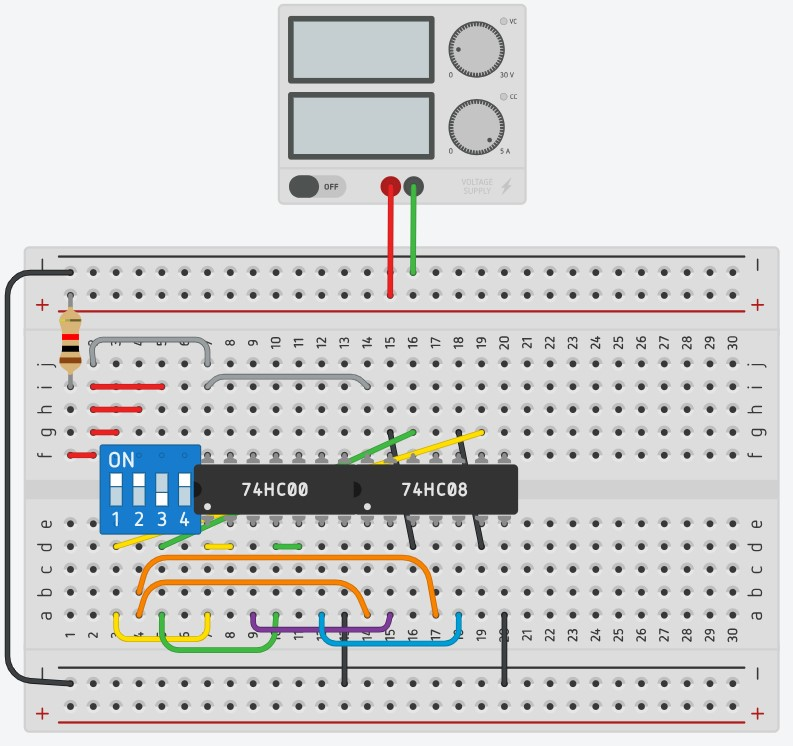
\includegraphics[scale=0.5]{Images/Tinkercad 04.jpg} \\
		\subsection{Porta Lógica OR (CI 7432)}
			Foi anexada na protoboard a porta lógica OR. Com 2 entradas, uma para cada sinal da Porta AND anterior.\\
			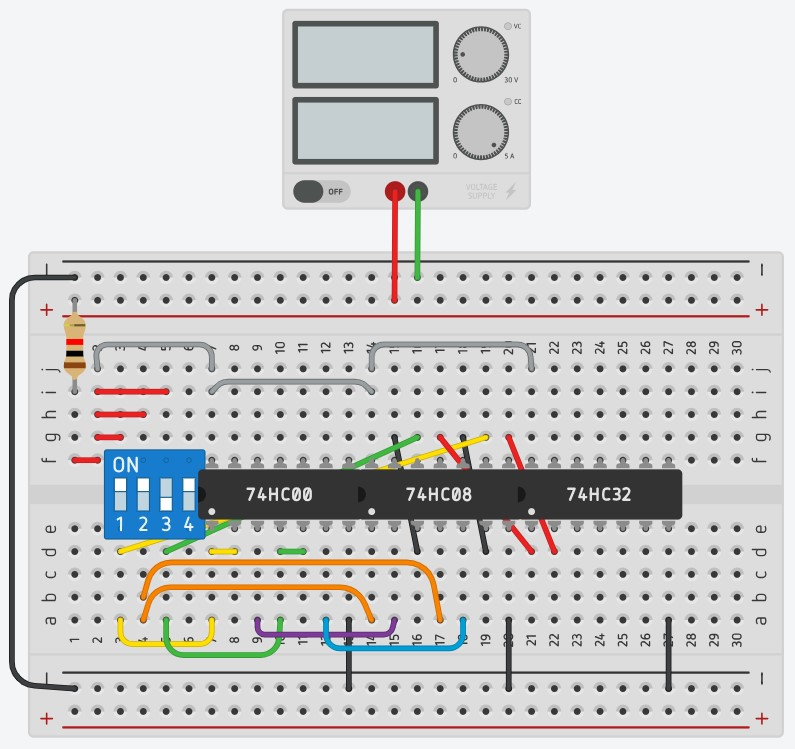
\includegraphics[scale=0.5]{Images/Tinkercad 05.jpg} \\
		\subsection{LED}
			A saída da porta lógica OR anterior foi ligada a um LED devidamente aterrado. Esse Led simula o Alarme do carro, quando está ligado o alarme dispara. \\
			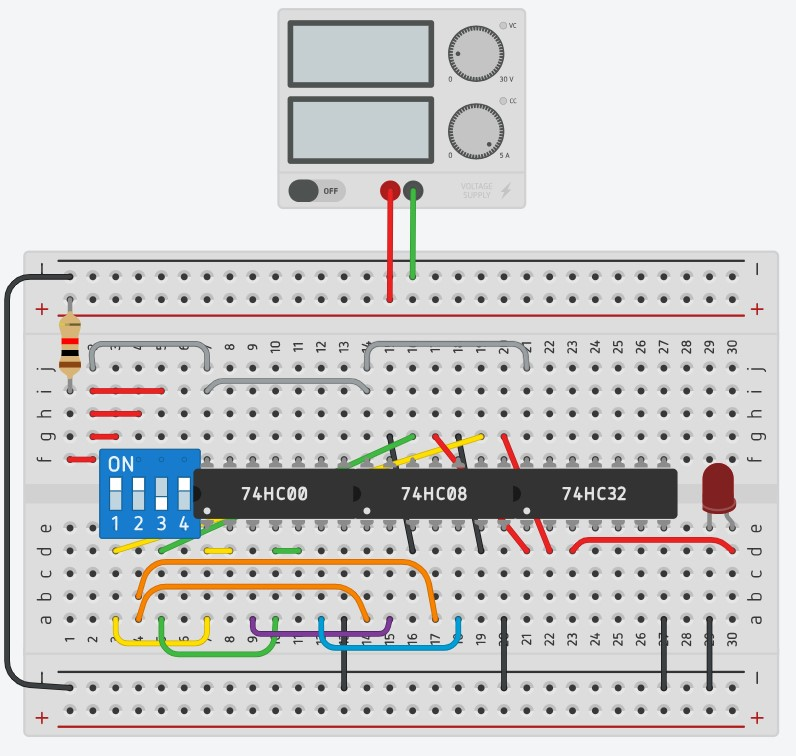
\includegraphics[scale=0.5]{Images/Tinkercad 06.jpg} \\
		\pagebreak
	\section{Circuito na Protoboard}
		\subsection{Mapeamento dos cabos}
			Os cabos que ligam a protoboard à fonte estão na linha horizontal inferior esquerda da protoboard; a linha de cima é o positivo e a de baixo o negativo. Na parte que liga a linha da esquerda com a direita foi usado um resistor como ponte e dali foi puxado um fio para uma linha vertical à esquerda do switch que foi usado para energizar as outras partes do circuito. \\ \\
			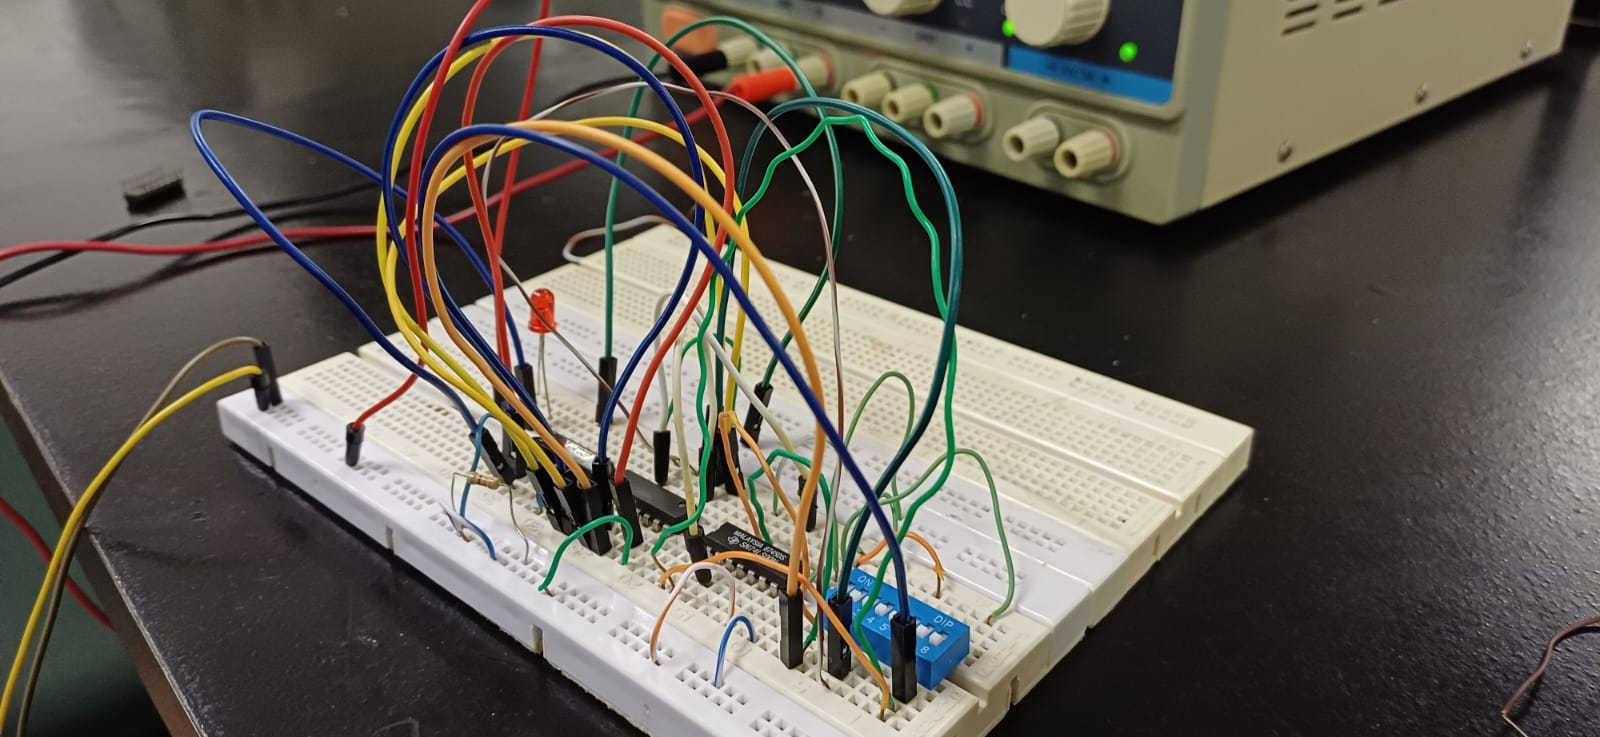
\includegraphics[scale=0.25]{Images/Protoboard Side.jpeg} \\
			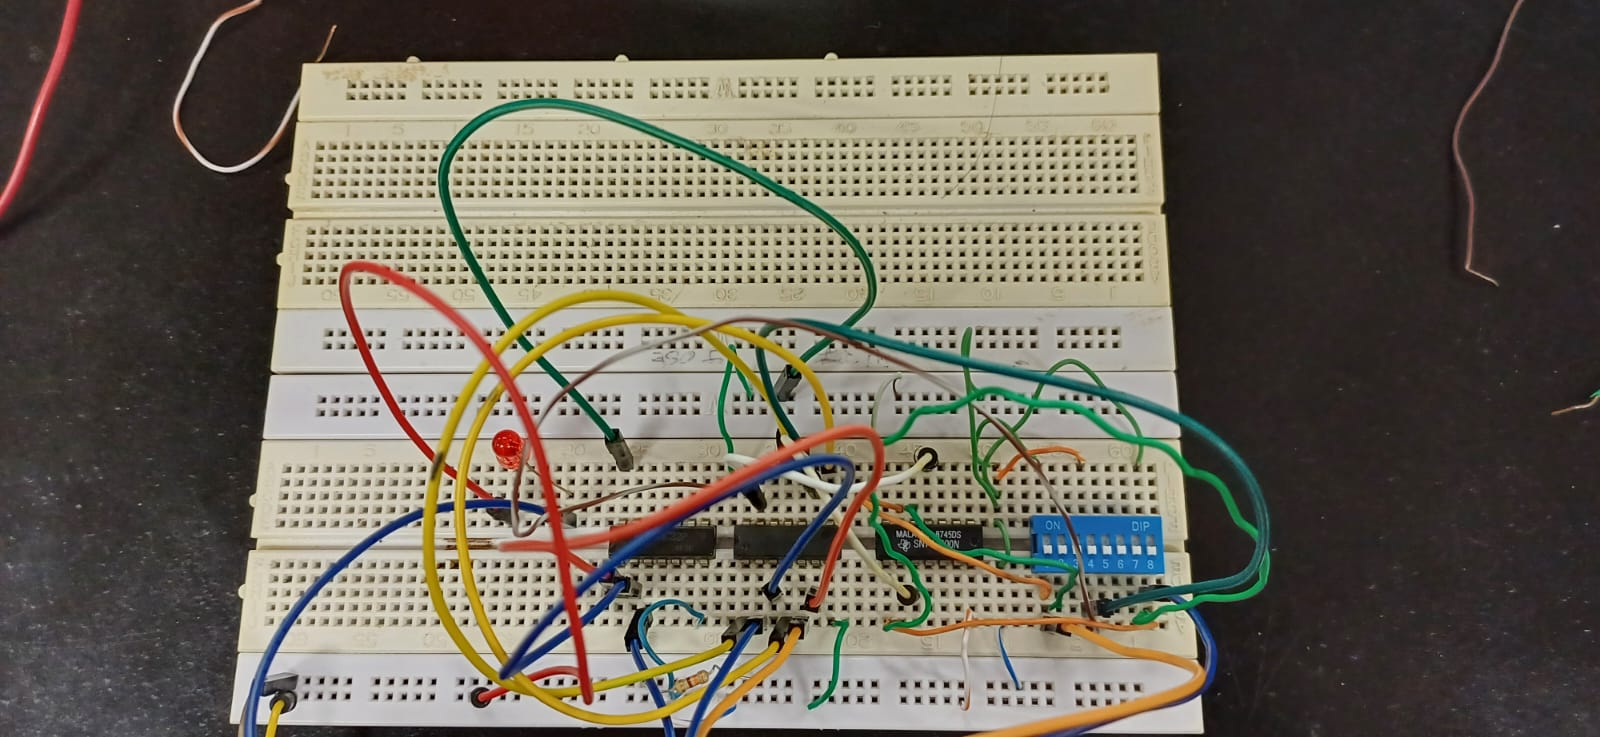
\includegraphics[scale=0.25]{Images/Protoboard Top.jpeg} \pagebreak\\
			Na porta AND, diferentemente do modelo apresentado no Tinkercad, foram puxados os fios priemeiro na parte superior para depois, na parte inferior, passarem por outra porta AND. Outra coisa que o circuito físico está diferente do circuito digital na plataforma virtual é que este foi montado da esquerda para a direita, com o switch à esquerda e o LED à direita. Já na protoboard, o circuito foi montado da direita para a esquerda. \\ \\
			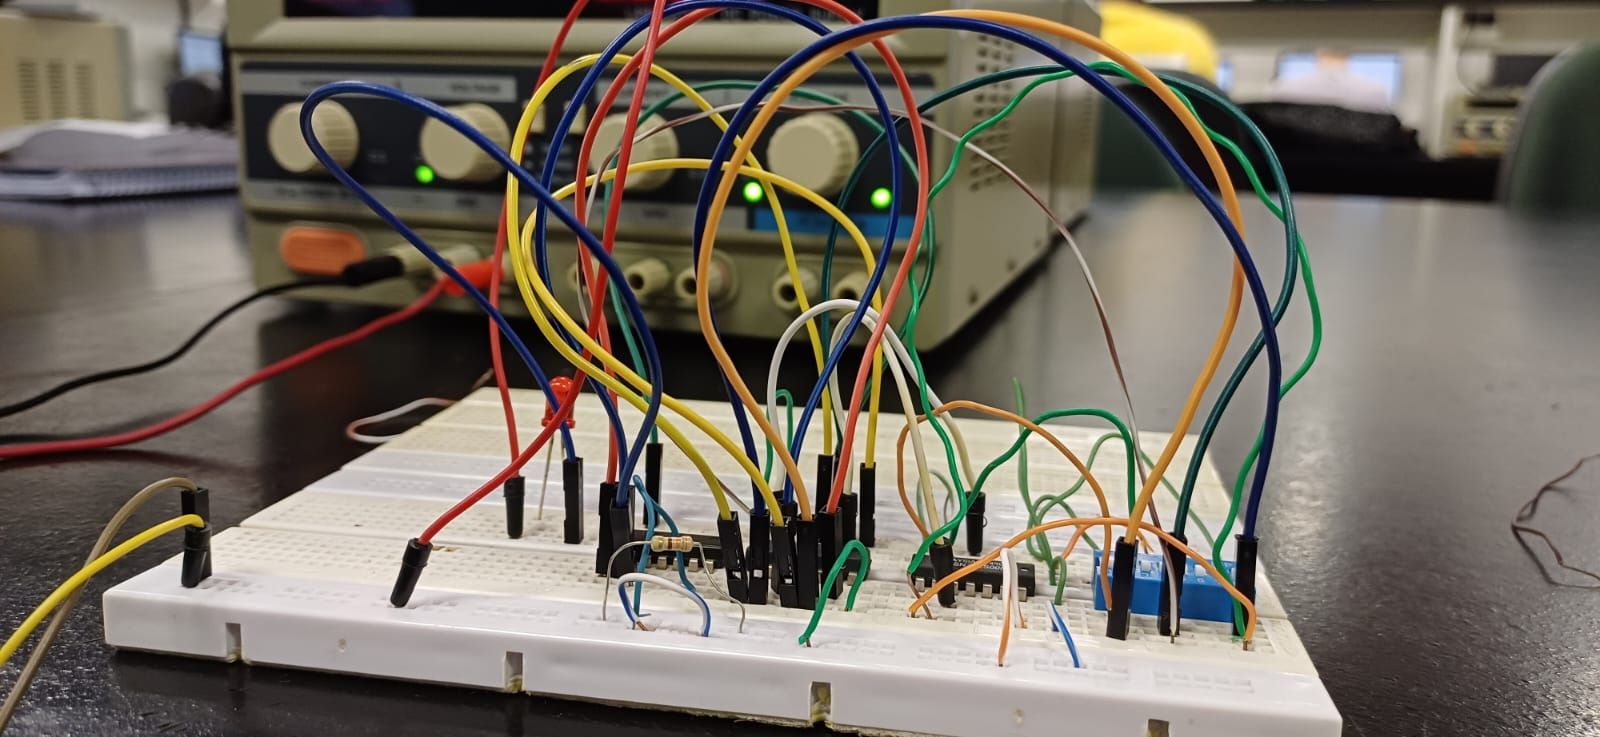
\includegraphics[scale=0.25]{Images/Protoboard Jumpers.jpeg} \\
			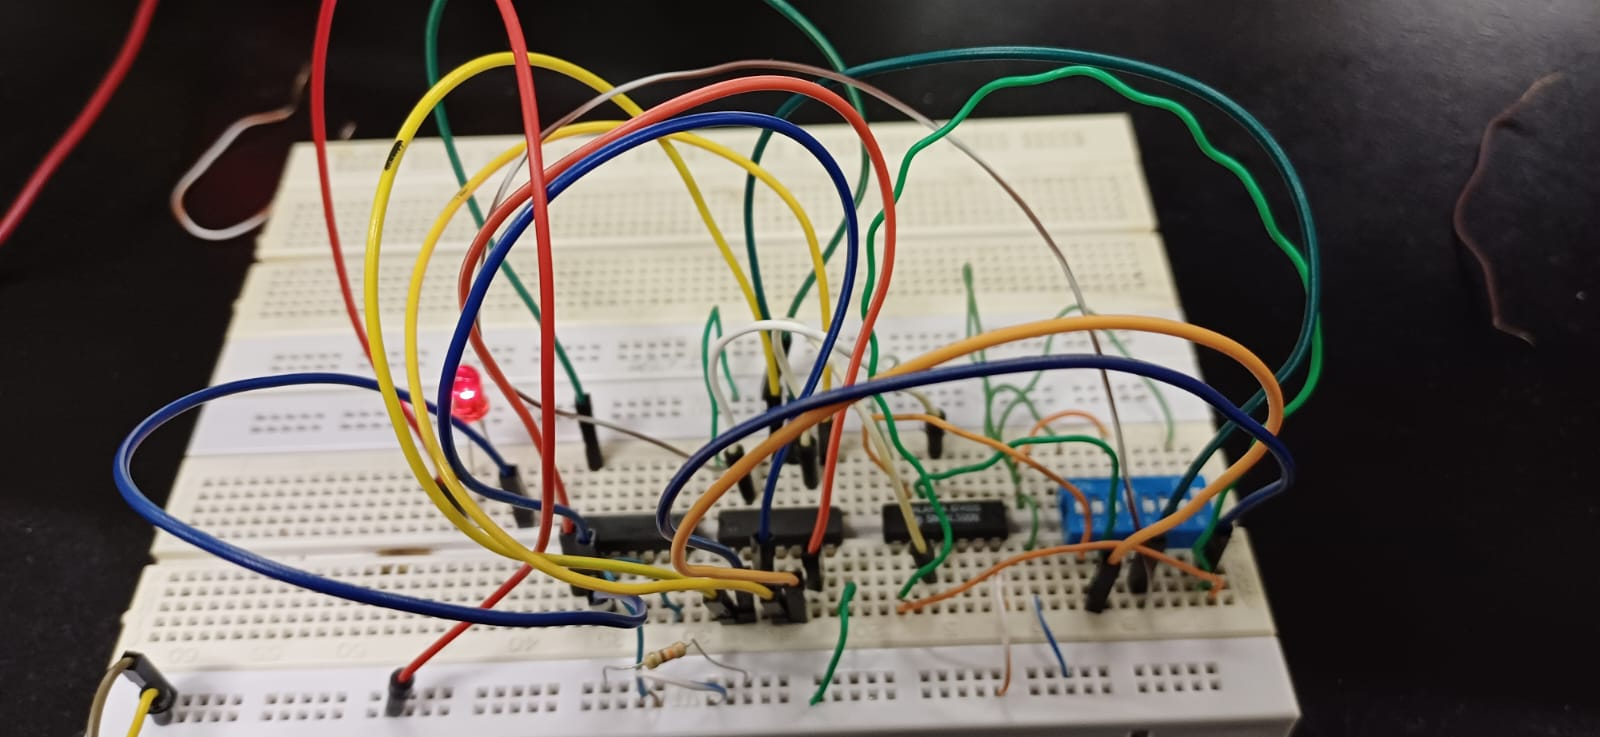
\includegraphics[scale=0.25]{Images/Protoboard Jumpers 2.jpeg} \\
		\subsection{(Farol, Porta, Chave) = (0,0,0) [Alarme Desativado]}
			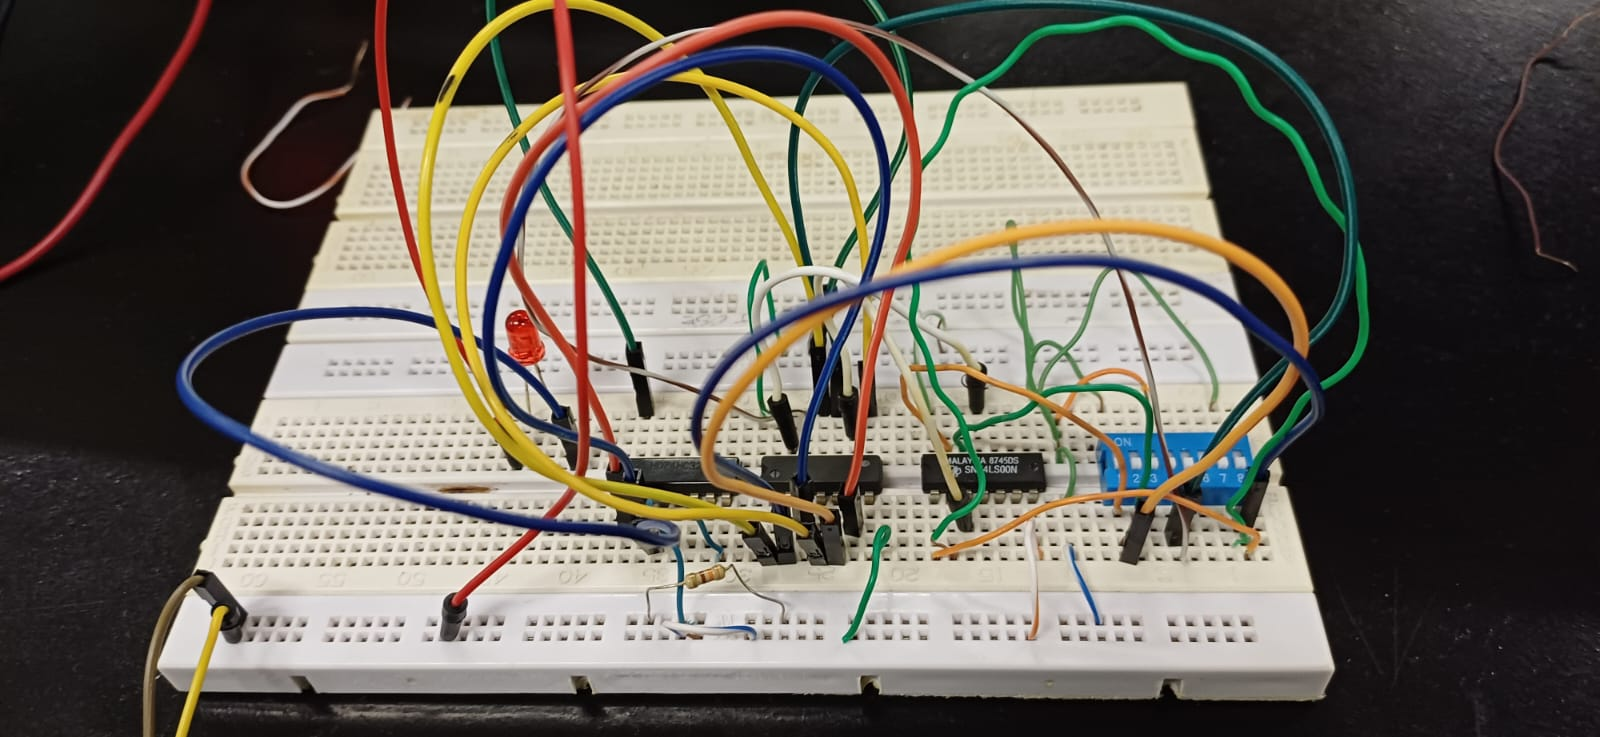
\includegraphics[scale=0.25]{Images/Protoboard 000 Down.jpeg} \\
			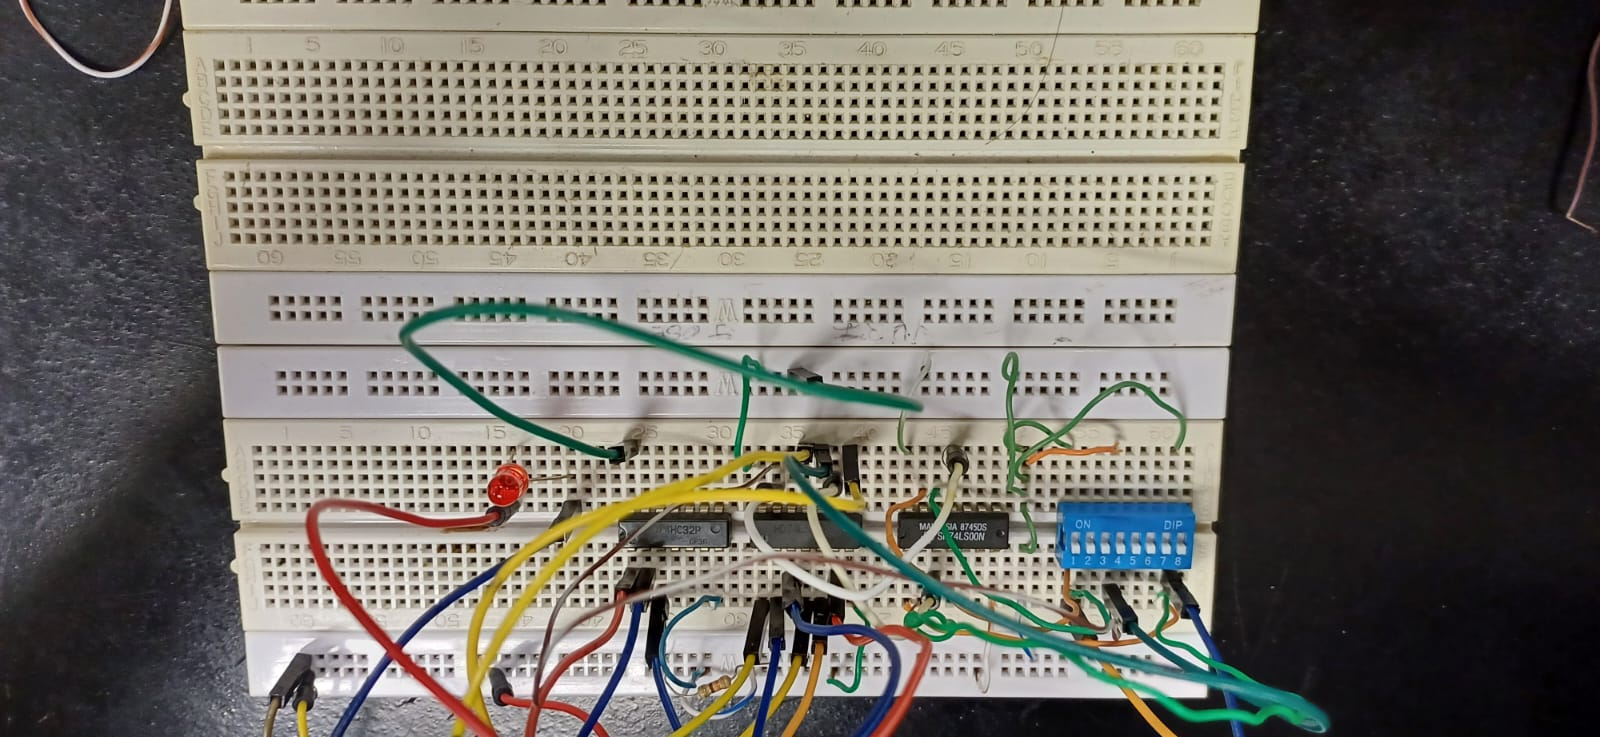
\includegraphics[scale=0.25]{Images/Protoboard 000 Top.jpeg} \\
		\subsection{(Farol, Porta, Chave) = (0,1,1) [Alarme Ativado]}
			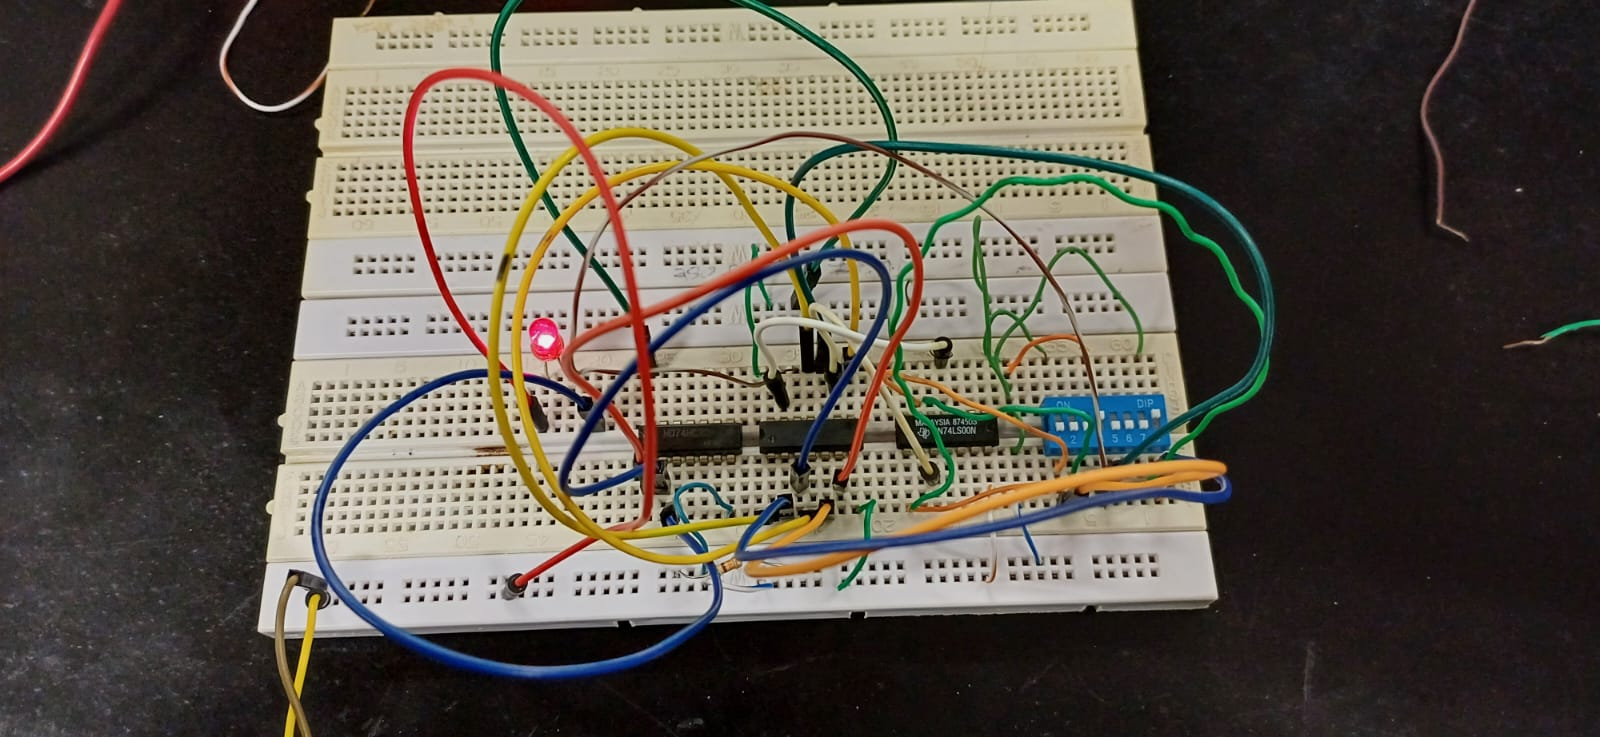
\includegraphics[scale=0.25]{Images/Protoboard 011 Down.jpeg} \\
			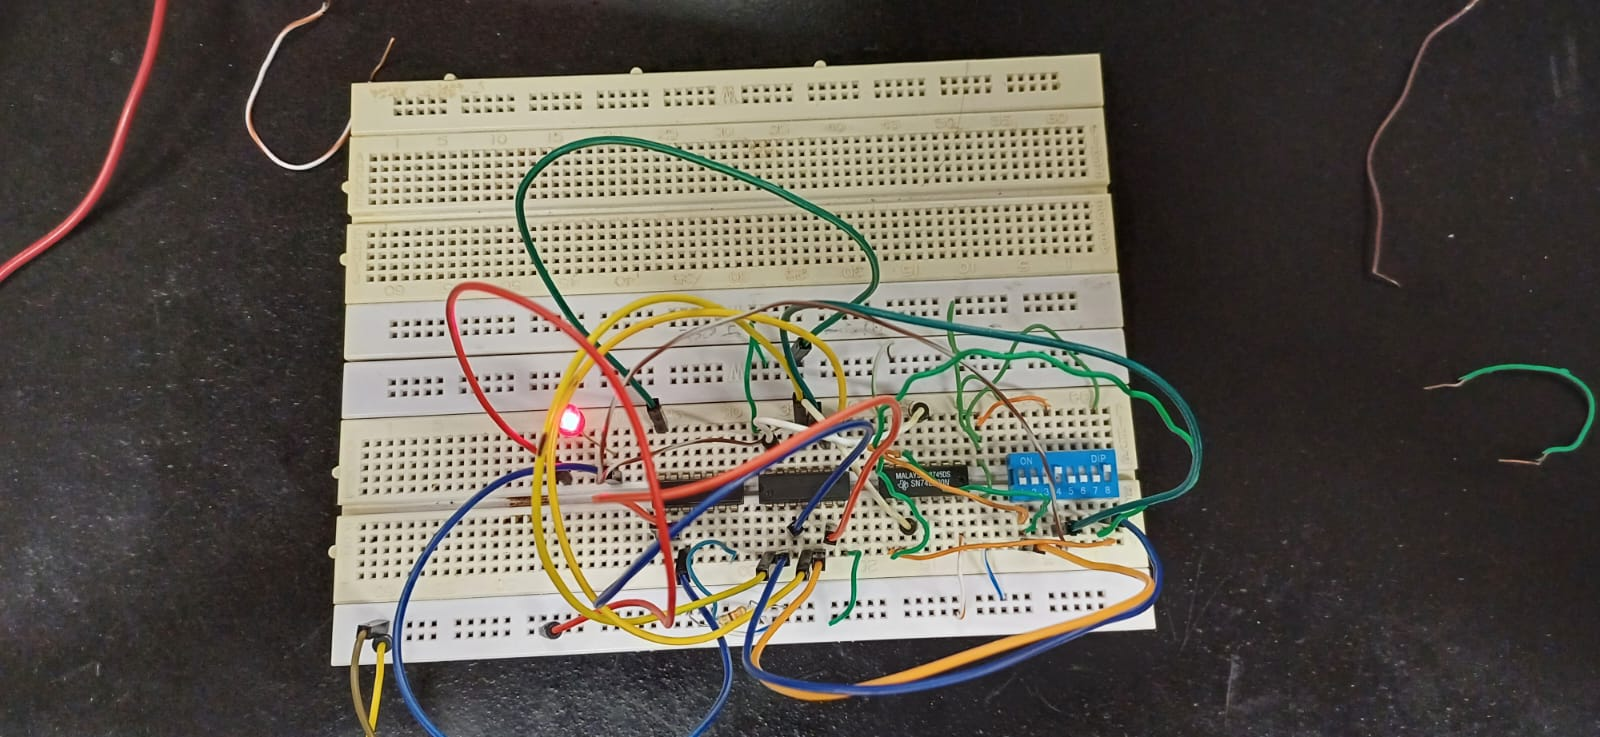
\includegraphics[scale=0.25]{Images/Protoboard 011 Top.jpeg} \\
		\subsection{(Farol, Porta, Chave) = (1,1,0) [Alarme Ativado]}
			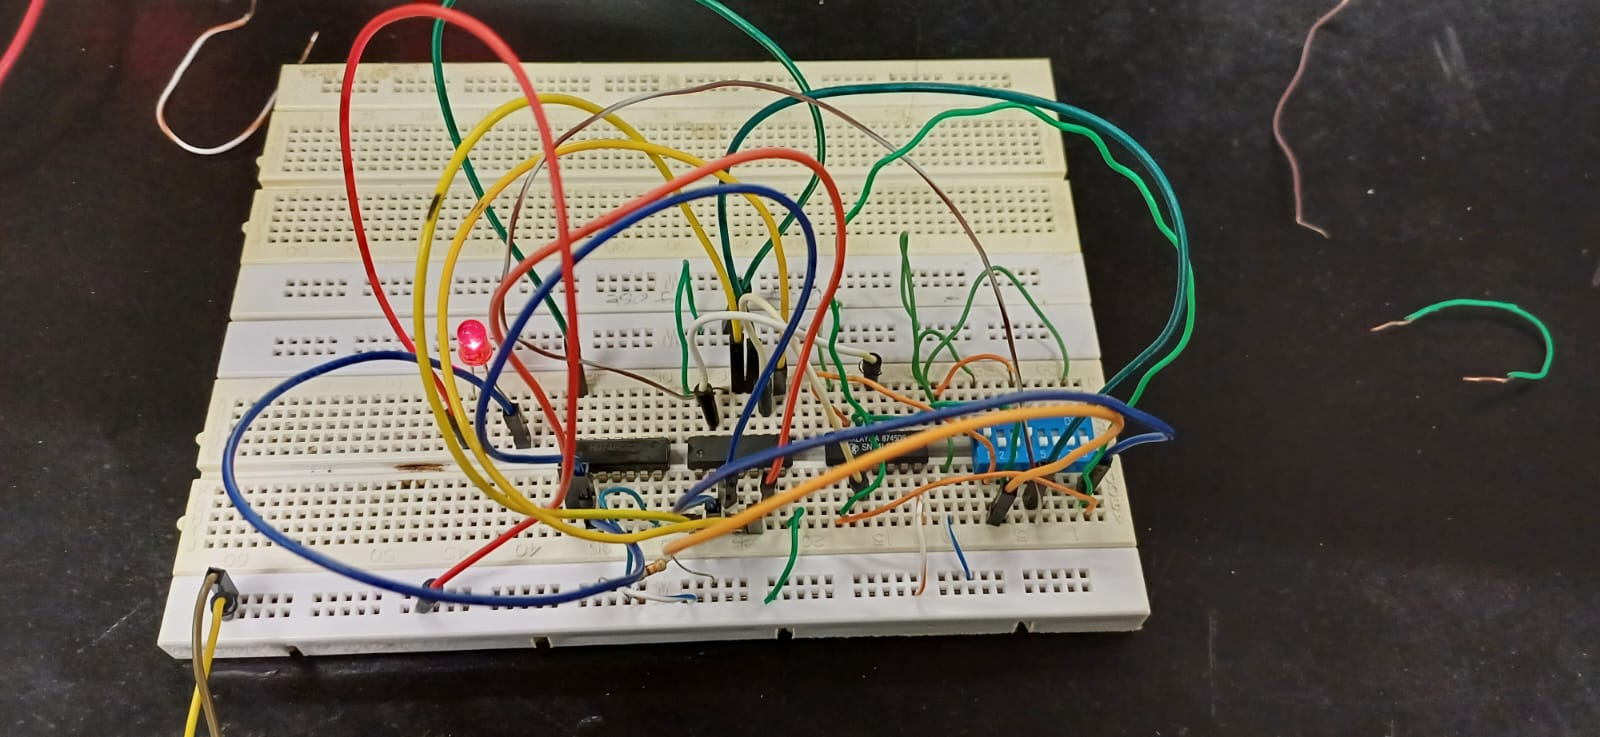
\includegraphics[scale=0.25]{Images/Protoboard 110 Down.jpeg} \\
			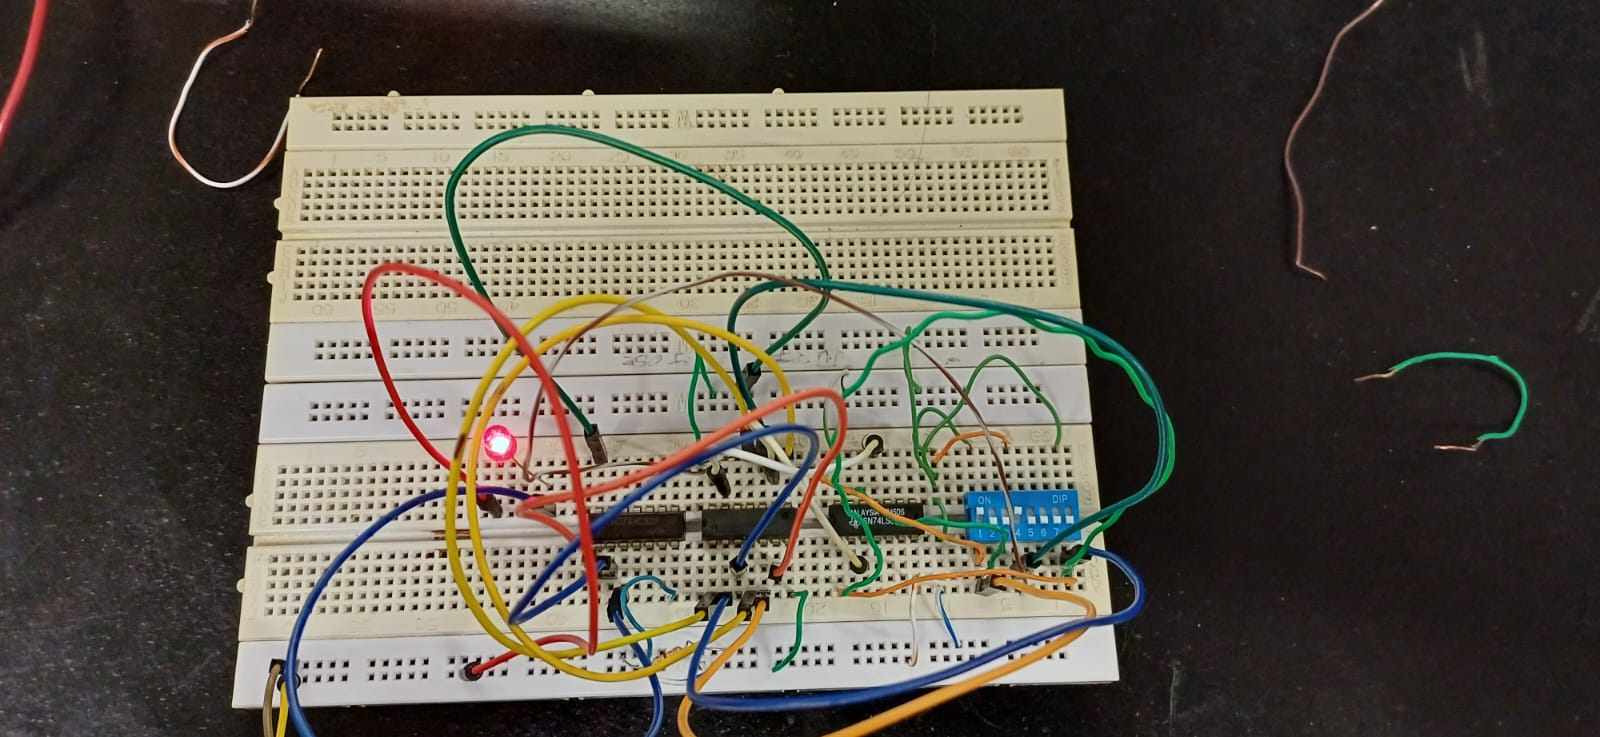
\includegraphics[scale=0.25]{Images/Protoboard 110 Top.jpeg} \\
		\subsection{(Farol, Porta, Chave) = (1,1,1) [Alarme Desativado]}
			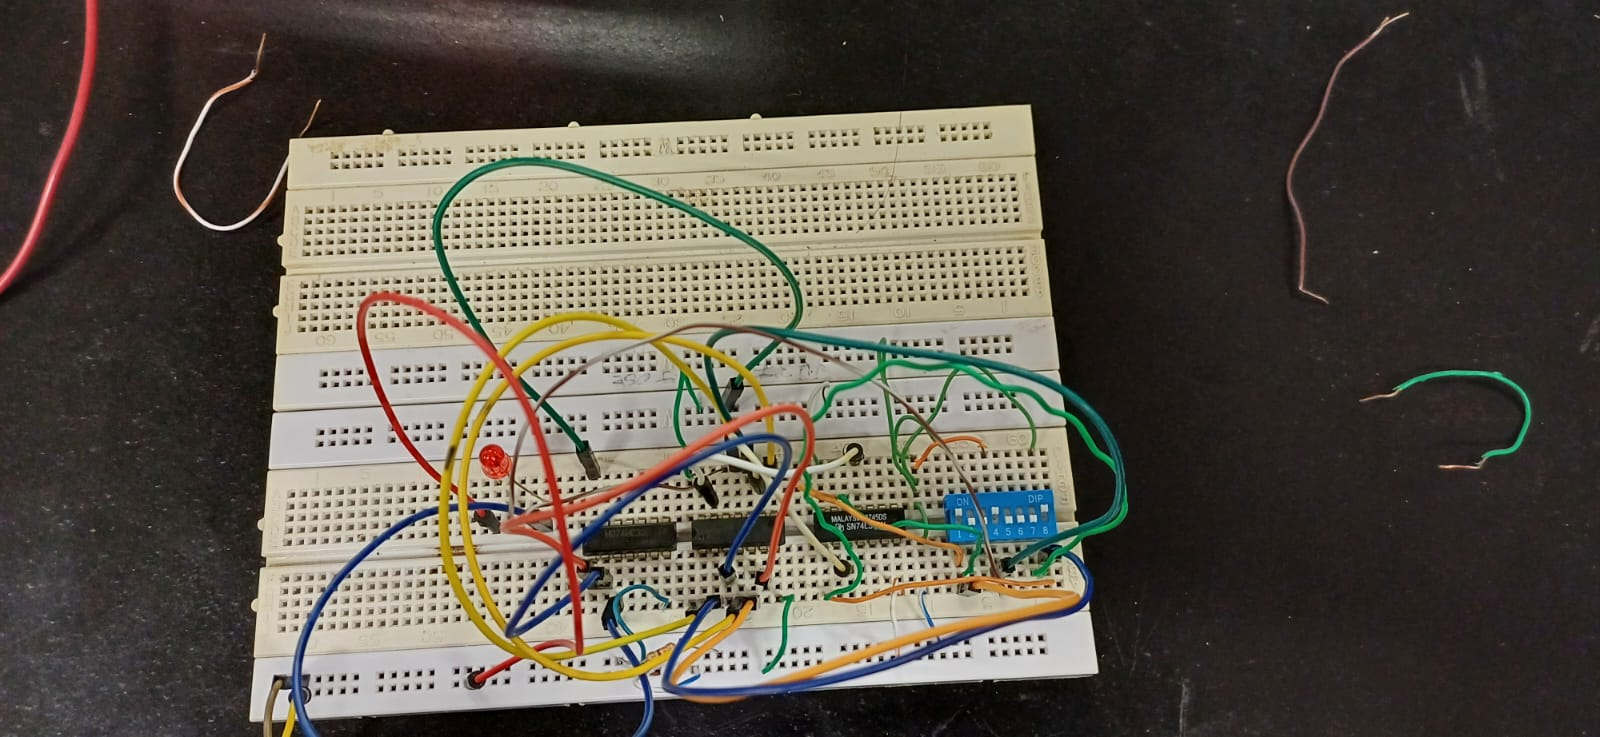
\includegraphics[scale=0.25]{Images/Protoboard 111 Down.jpeg} \\
		
\end{document}